\documentclass{beamer}

\usepackage{fontspec}
\usepackage{xltxtra}
\usepackage{graphicx}
\usepackage{animate}
\usepackage{subfig}
\usepackage{appendixnumberbeamer}

\mode<presentation>{
  \useoutertheme{shadow}
  \usetheme{Singapore}
  \setbeamertemplate{items}[circle square]
  \setbeamertemplate{navigation symbols}{}%remove navigation symbols
  \setbeamerfont{block title}{size={}}
  \setbeamercovered{dynamic}
}

\setbeamertemplate{footline}
{
  \leavevmode%
  \hbox{%
  \begin{beamercolorbox}[wd=.3\paperwidth,ht=2.25ex,dp=1ex,center]{institute in head/foot}%
    \usebeamerfont{author in head/foot}\insertshortinstitute\hspace*{10em}
  \end{beamercolorbox}%
  \begin{beamercolorbox}[wd=.6\paperwidth,ht=2.25ex,dp=1ex,center]{title in head/foot}%
    \usebeamerfont{title in head/foot}\insertshorttitle\hspace*{10em}
    \insertframenumber{} / \inserttotalframenumber\hspace*{1ex}
  \end{beamercolorbox}}%
  \vskip0pt%
}

\title{High performance shared state schedulers}
\author[AK]{Antonios Kouzoupis\\[1em]{\footnotesize Examiner: Jim
    Dowling\\Supervisors: Seif Haridi, Gautier Berthou}}
\institute[KTH/SICS]{}

\titlegraphic{
\includegraphics[scale=0.15]{resources/KTH_logo.eps}~

\includegraphics[scale=0.15]{resources/SICS_logo.eps}}

\date[date]{August 19, 2016}

\setsansfont[Mapping=tex-text]{GFS Didot}
\setmonofont[Mapping=tex-text, Scale=0.6]{GFS Didot}
\font\mono="DejaVu Sans Mono" at 9pt

\begin{document}

\section{}
\begin{frame}
\titlepage
\end{frame}

\section*{}
\begin{frame}
\frametitle{Outline}
\footnotesize
\tableofcontents
\normalsize
\end{frame}

\section{Introduction}
\subsection{Hadoop}
\begin{frame}
\frametitle{Apache Hadoop}
Open-source framework for distributed storage and processing of large
datasets across clusters of computers
\begin{itemize}
\item \textbf{Hadoop Distributed File System (HDFS)}
\item \textbf{Hadoop YARN}
\item Apache MapReduce
\item Apache Flink
\item Apache HBase
\item ...
\end{itemize}
\end{frame}

\begin{frame}
\frametitle{Apache YARN}
Mainly consists of three entities:
\begin{enumerate}
\item<+-> \emph{ResourceManager} Central authority for scheduling
  decisions and allocation of resources, handles heartbeats from NM
  and AM, tracks their liveness

\item<+-> \emph{NodeManager} Per-node ``worker'' daemon, monitoring the
  health of the machine, responsible for application
  containers. Heartbeats periodically the RM

\item<+-> \emph{ApplicationMaster} Per-application process
  coordinating the execution plan of the job, requesting or releasing
  containers and monitors containers
\end{enumerate}
\end{frame}

\begin{frame}
\frametitle{Apache YARN architecture}
\begin{figure}
\centering
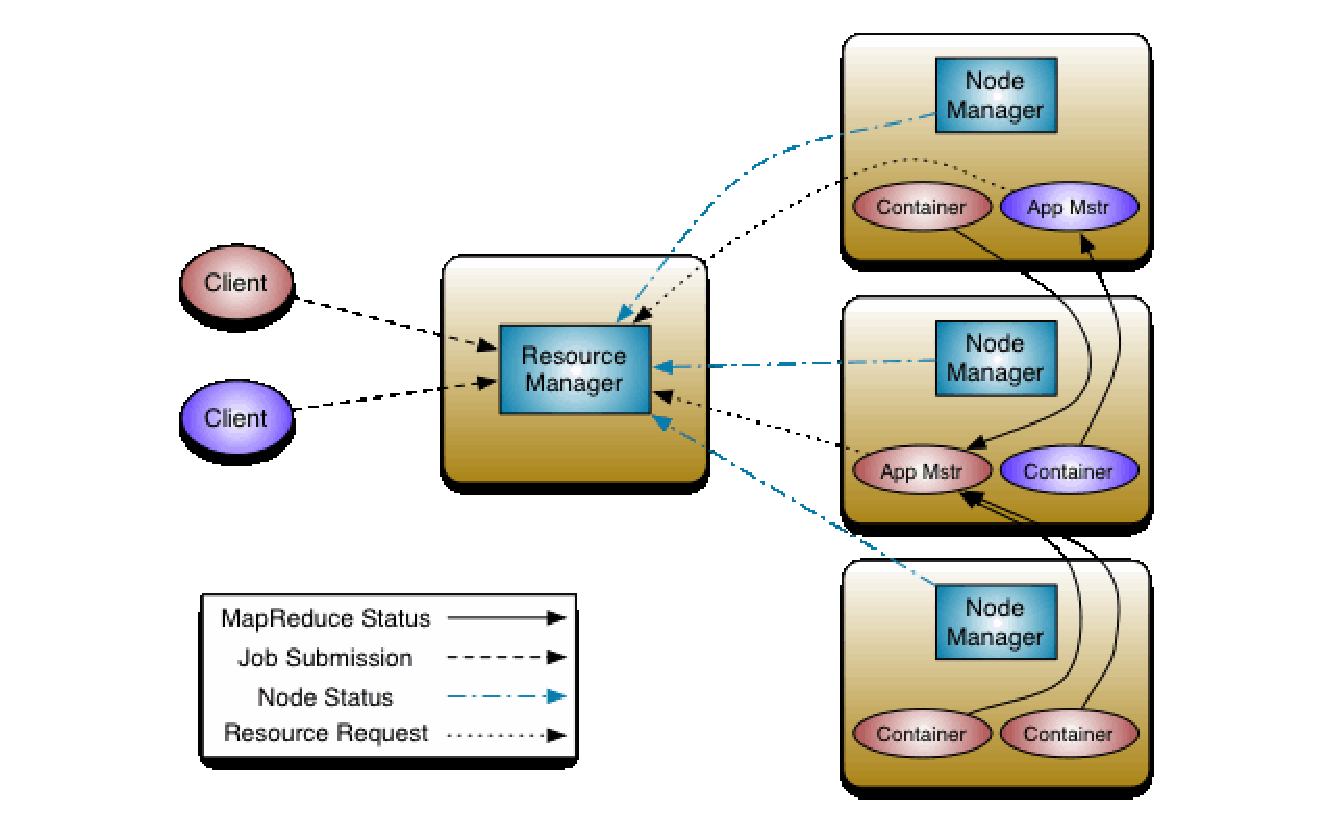
\includegraphics[scale=0.4]{resources/yarn_architecture.eps}
\end{figure}
\tiny{*https://hadoop.apache.org/docs/r2.7.1/hadoop-yarn/hadoop-yarn-site/YARN.html}
\end{frame}

\begin{frame}
\frametitle{HA \& failure recovery}
\begin{itemize}
\item Multiple RMs in an active/standby architecture coordinated by
  Apache ZooKeeper

\item Store applications' state in a persistent storage, usually
  ZooKeeper

\item When a RM transitions from standby to active, reads the state
  from ZooKeeper and asks \textbf{every} NM and AM to resync
\end{itemize}
\end{frame}

\subsection{Hops}
\begin{frame}
\frametitle{Hops stack}
Hops is a new distribution of Apache Hadoop with:
\begin{itemize}
\item \emph{HopsWorks}, a web UI for Hops platform
\item \emph{HopsFS} customized HDFS with distributed NameNodes
\item \textbf{HopsYARN} customized, highly available version of Apache
  YARN, with distributed ResourceTrackers and minimum recovery time
\item Other services like Kafka, Dr. Elephant, etc
\end{itemize}
\end{frame}

\begin{frame}
\frametitle{Hops-YARN}

\begin{itemize}
\item Persist RM state in a distributed MySQL Cluster NDB

\item Persist every single heartbeat from AM/NM and subsequent responses

\item<2-> Standby is boring! Standby RMs act as ResourceTrackers
  receiving heartbeats from NM, load balacing the active RM
\end{itemize}
\end{frame}

\begin{frame}
\frametitle{Hops-YARN architecture I}

\begin{figure}
\centering
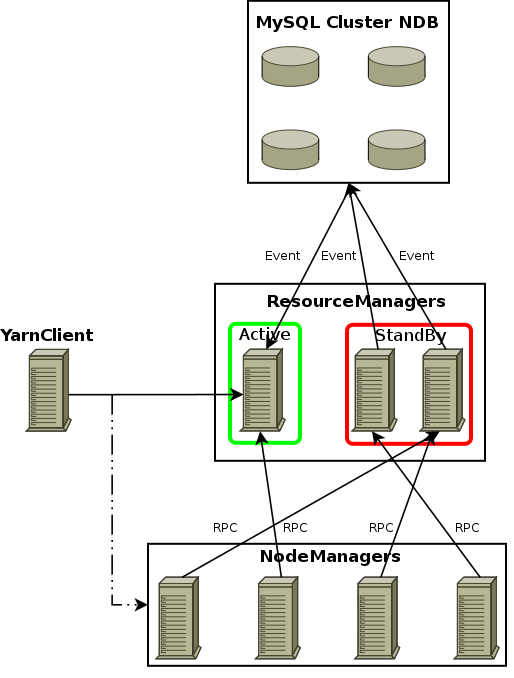
\includegraphics[scale=0.3]{resources/hopsyarn_arch_overview.png}
\end{figure}
\end{frame}

\begin{frame}
\frametitle{Hops-YARN architecture II}

\begin{figure}
\centering
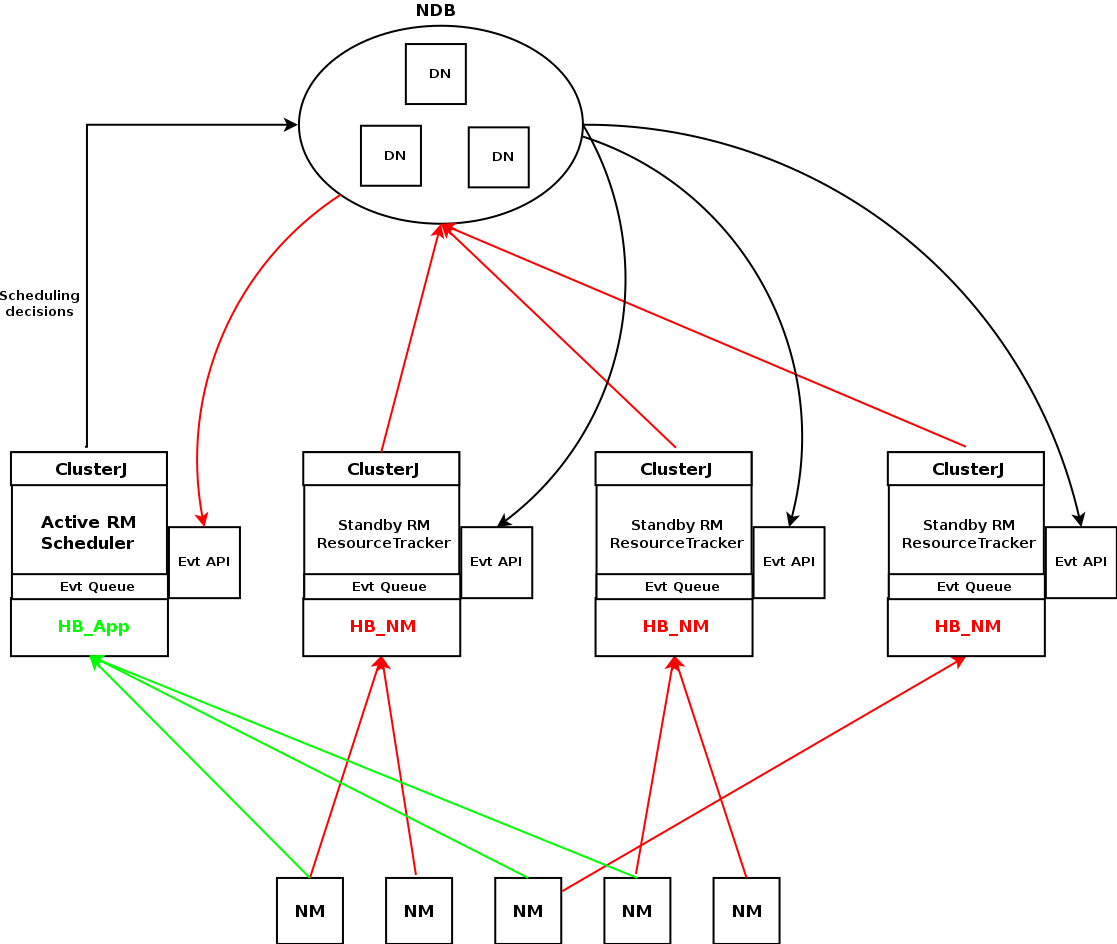
\includegraphics[scale=0.17]{resources/hopsyarn_arch_components.png}
\end{figure}
\end{frame}


\begin{frame}
\frametitle{MySQL Cluster}
\begin{itemize}
\item In-memory clustered storage engine NDB
\item ACID compliant
\item Transactional
\item Row-level locking
\item Shared-nothing architecture
\item No single point of failure
\end{itemize}
\end{frame}

\begin{frame}
\frametitle{Shared state schedulers}
\textbf{\underline{Multiple}} schedulers running \textbf{\underline{different}} scheduling
policies, operating on the \textbf{\underline{full view}} of the cluster.
\begin{itemize}
\item Optimistic concurrency control to increase scheduler parallelism
\item Shared persistent storage for the allocations in the cluster
\item Each scheduler operates on a local, frequently synced copy
\item Atomic commit, at most one transaction will succeed
\end{itemize}
\end{frame}

\section{Implementation}
\subsection{Foreign key constraints}
\begin{frame}
\frametitle{Foreign Key constraints}
Relational database feature that uniquely identifies a field in one
table with a row in another table.\\[2em]

In Hops we use them mainly for the \texttt{ON DELETE CASCADE}
referential action.

\begin{enumerate}
\item {\color{red} Great} performance overhead
\item Serialization of operations, a lot of {\color{red} flushes}
\end{enumerate}
\end{frame}

\begin{frame}
\frametitle{Foreign Key constraints}
\begin{figure}
\centering
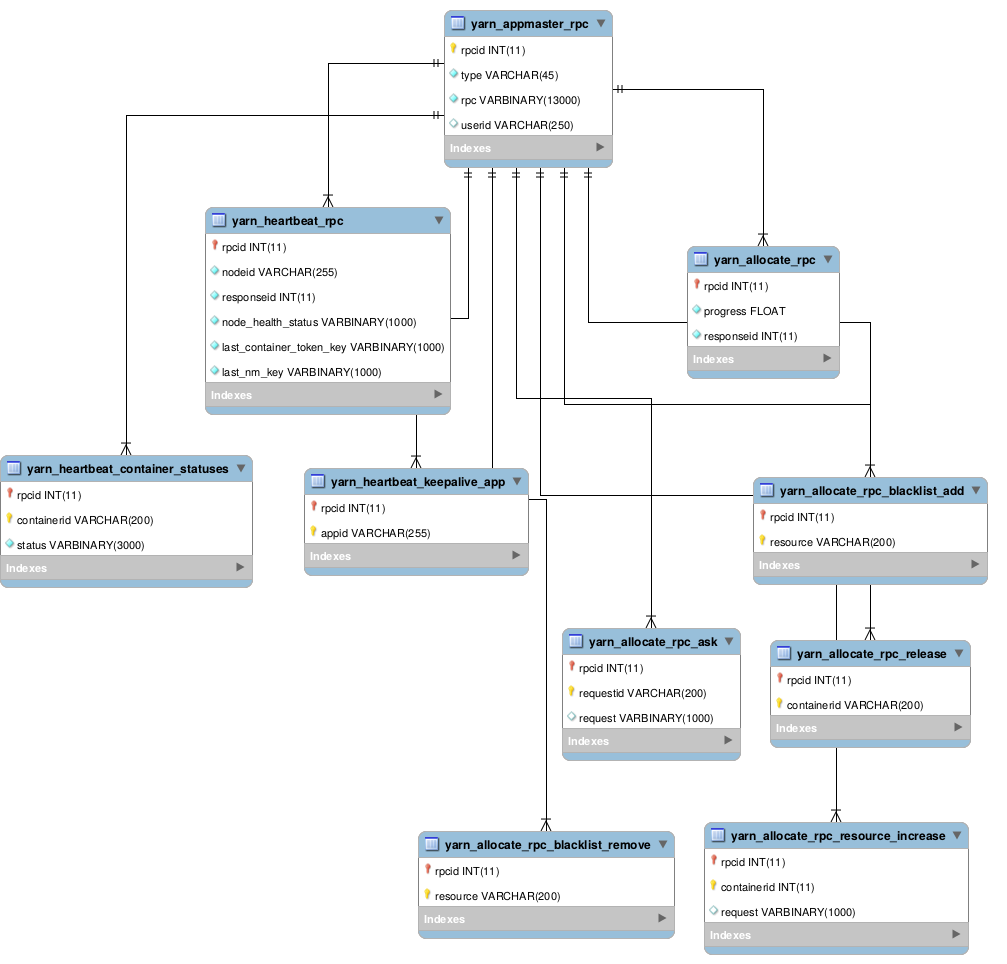
\includegraphics[scale=0.18]{resources/hops_yarn_ndb_schema_rpc.png}
\caption{Schema to store RPCs}
\end{figure}
\end{frame}

\begin{frame}
\frametitle{Foreign Key constraints}
\begin{figure}
\centering
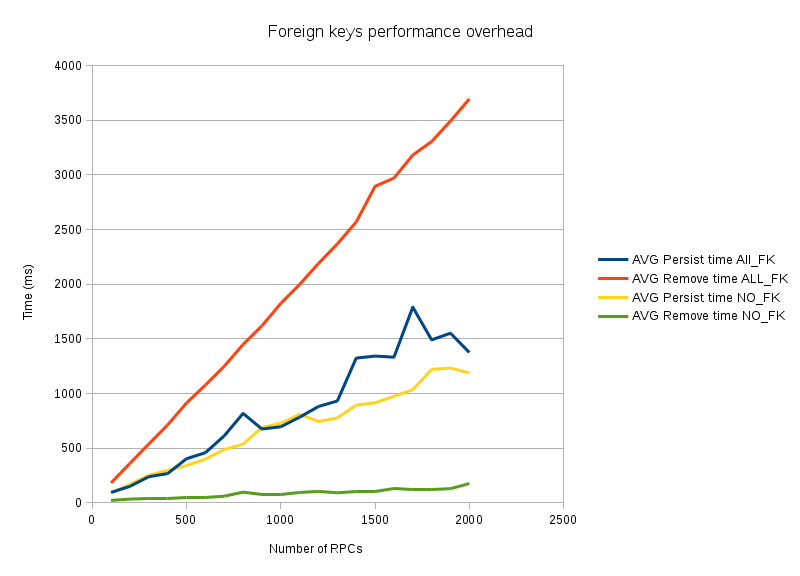
\includegraphics[scale=0.4]{resources/fk_overhead.png}
\caption{Foreign key constraints overhead}
\end{figure}
\end{frame}

\begin{frame}
\frametitle{Solution}
Replace all foreign key constraints with application logic that makes
\textbf{primary key} operations.

\begin{itemize}
\item<+-> Primary keys are indexed in B-tree data structures, allows
  operations in $O(\log{}n)$
\item<+-> Primary keys in NDB are partition keys, avoid RTT among Data
  Nodes
\end{itemize}
\end{frame}

\subsection{Transaction State aggregation}
\begin{frame}
\frametitle{Transaction State}

\begin{enumerate}
\item RPCs arrive in RM
\item The method invoked triggers appropriate events
\item Events are handled by RM components changing some state
\item Components might trigger other events
\item Scheduler at the same time makes scheduling decisions
\end{enumerate}

\pause
\vfill
\centering
{\color{red} How do we track the changes in a consistent way?}
\end{frame}

\begin{frame}
\frametitle{Transaction State}
A \emph{Transaction State} object tracks all the modifications
introduced by the RPCs, the scheduling decisions or Events from NDB

\begin{enumerate}
\item The method invoked gets that object and piggybacks it to the
  events triggered
\item Each time a modification happens to the state of RM, we record
  it in the TS data structures
\item The same object travels all along the RM
\item When all events have been handled we put it in a \textbf{waiting
    queue}, create a new TS object and a separate thread \textbf{tries} to commit in NDB
\end{enumerate}

\pause
\vfill
\centering
{\color{red} How do we guarantee that two conflicting TSs are
  committed in the correct order?}
\end{frame}

\begin{frame}
\frametitle{Commit mechanism}
Three rules followed:

\begin{itemize}
\item<1,4> If \emph{TS$_0$} has been placed in the waiting queue before
  \emph{TS$1$} and they both modify the same \textbf{application},
  then the commit phase of \emph{TS$_0$} should have been successfully
  completed \textbf{before} the commit phase of \emph{TS$_1$} begins.

\item<2,4> If \emph{TS$_0$} has been placed in the waiting queue before
  \emph{TS$1$} and they both modify the same \textbf{NodeManager},
  then the commit phase of \emph{TS$_0$} should have been successfully
  completed \textbf{before} the commit phase of \emph{TS$_1$} begins.

\item<3,4> If \emph{TS$_0$} and \emph{TS$_1$} modify different
  applications \textbf{and} different NodeManagers then they should be
  committed in parallel
\end{itemize}
\end{frame}

\begin{frame}
\frametitle{Commit mechanism}

\begin{figure}
\centering
\only<1>{
  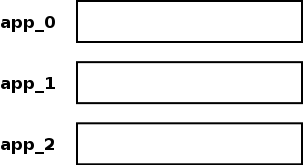
\includegraphics[scale=0.5]{resources/commit_system_0.png}
}
\only<2>{
  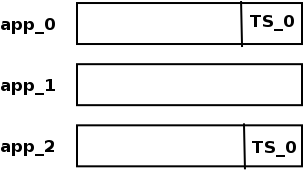
\includegraphics[scale=0.5]{resources/commit_system_1.png}
}
\only<3>{
  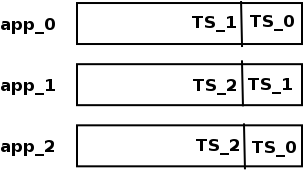
\includegraphics[scale=0.5]{resources/commit_system_2.png}
}
\only<4>{
  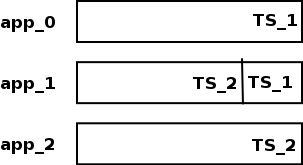
\includegraphics[scale=0.5]{resources/commit_system_3.png}
}
\only<5>{
  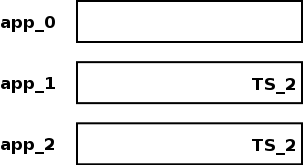
\includegraphics[scale=0.5]{resources/commit_system_4.png}
}

\caption{Locking system}
\end{figure}
\end{frame}

\begin{frame}
\frametitle{Commit mechanism}

The current system guarantees order of TSs and parallelism but

\begin{enumerate}
\item TSs are blocked in the queue by conflicting TS
\item For each TS we pay the network latency penalty
\end{enumerate}
\end{frame}

\begin{frame}
\frametitle{Aggregation mechanism}
\emph{AggregatedTransactionState} extends the TS object and aggregates
two or more TSs ensuring the order of modifications.

Maintain the existing system but aggregate blocked TSs according to
two \emph{aggregation rules}

\begin{itemize}
\item<+-> A TS was not the head in its respective queues at the time
  it was examined for commit, but until now the conflicting TS(s) have
  been committed and removed. So now it is in the head of the queues.

\item<+-> A TS is still not in the head of its respective queues, but
  the conflicting TSs that should be committed before, have already
  been aggregated in the \emph{AggregatedTransactionState}
\end{itemize}
\end{frame}

\begin{frame}
\frametitle{Aggregation mechanism}

\begin{figure}
\centering
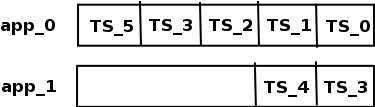
\includegraphics[scale=0.5]{resources/commit_system_aggr_example.png}
\caption{Aggregation example}
\end{figure}
\end{frame}

\begin{frame}
\frametitle{Aggregation policy}
By aggregating several TS we ended up overloading NDB and made
transactions fail. Solve this issue by an adaptive aggregation policy
that:

\begin{itemize}
\item Increase the aggregation limit by a factor every time an
  \emph{AggregatedTransactionState} transaction finishes successfully
\item Reset the aggregation limit to minimum every time an
  \emph{AggregatedTransactionState} transaction fails with a specific error
\end{itemize}

\end{frame}
\subsection{Garbage Collector service}
\begin{frame}
\frametitle{GC service}

Some operations in the TransactionState still take time to finish
prolonging the commit time and delaying other blocked TSs

\begin{description}
\item[RPC] Delete operation on 10 tables with FK constraint,
  \texttt{ON DELETE CASCADE} (I have not removed them for this set of tables)
\item[Allocate Response] Before persisting one Allocate Response,
  remove the previous from the database. So an insert operation,
  implicitely means an extra deletion operation
\end{description}
\end{frame}

\begin{frame}
\frametitle{GC service}

Instead of removing the old RPCs and Allocate Responses synchronously
in the Transaction State, persist \textbf{only} \texttt{<rpcid,type>}
and \texttt{<applicationattemptid,responseid,type>} of old RPCs and
Allocate Responses in GC tables. No \underline{delete} operations!\\[2em]

Old entries are removed \textbf{asynchronously} by the Garbage Collector
service run on Hops-YARN.
\end{frame}

\begin{frame}
\frametitle{GC service}

\begin{enumerate}
\item A \emph{worker} thread fetches old RPCs and Allocate Responses from the
  GC database tables

\item \emph{Worker} spawns threads performing delete operations on the
  appropriate tables storing RPCs and Allocate Responses, removing old
  values

\item When all the delete transactions successfully complete, remove
  the old ``keys'' from the GC tables

\item \texttt{GOTO} 1
\end{enumerate}
\end{frame}

\subsection{DTO caching mechanism}
\begin{frame}
\frametitle{DTO caching}
\end{frame}

\section{Results}
\begin{frame}
\frametitle{Results}
\end{frame}

\section{Conclusions}
\begin{frame}
\frametitle{Conclusions}
\end{frame}

\end{document}